\documentclass[14pt]{extarticle}
\usepackage[]{cite}
\usepackage{cmap}
\usepackage[T2A]{fontenc}
\usepackage[utf8]{inputenc}
\usepackage[english, russian]{babel}
\usepackage{amsmath, amsfonts,amssymb,mathrsfs}
\usepackage{graphicx, epsfig}
\usepackage{subfig}
% \usepackage{color}
\usepackage{algorithm}
\usepackage{algorithmic}
\usepackage{indentfirst}
\floatname{algorithm}{Алгоритм}
\usepackage[hidelinks]{hyperref}
\usepackage{xcolor}

%\hypersetup{
%	colorlinks,
%	linkcolor={red!50!black},
%	citecolor={blue!50!black},
%	urlcolor={blue!80!black}
%}

\usepackage{mathrsfs}
\usepackage{longtable}
\usepackage{wrapfig}
\usepackage{float}
\usepackage{subfloat}
\usepackage{caption}
\usepackage{multirow}
\usepackage{dsfont}
\graphicspath{{./img/}}
% \usepackage{xcolor}
% \usepackage[dvipsnames]{color}
%\usepackage[dvipsnames]{xcolor}
%\definecolor{mynicegreen}{RGB}{102,252,102}
\usepackage[labelsep=endash]{caption}

\newcommand\argmin{\mathop{\arg\min}}
\DeclareMathOperator*{\argmax}{argmax}
\newcommand{\T}{^{\text{\tiny\sffamily\upshape\mdseries T}}}
\newcommand{\hchi}{\hat{\boldsymbol{\chi}}}
\newcommand{\hphi}{\hat{\boldsymbol{\varphi}}}
\newcommand{\bchi}{\boldsymbol{\chi}}
\newcommand{\A}{\mathcal{A}}
\newcommand{\B}{\mathcal{B}}
\newcommand{\x}{\mathbf{x}}
\newcommand{\hx}{\hat{x}}
\newcommand{\hy}{\hat{y}}
\newcommand{\M}{\mathcal{M}}
\newcommand{\N}{\mathcal{N}}
\newcommand{\R}{\mathbb{R}}
\newcommand{\p}{p(\cdot)}
\newcommand{\q}{q(\cdot)}
\newcommand{\uu}{\mathbf{u}}
\newcommand{\vv}{\mathbf{v}}


\renewcommand{\baselinestretch}{1}

%\textheight=22cm % высота текста
%\textwidth=16cm % ширина текста
%\oddsidemargin=40pt % отступ от левого края
%\evensidemargin=15pt % отступ от правого края
%\topmargin=-20mm % отступ от верхнего края
%\parindent=24pt % абзацный отступ
%\parskip=5pt % интервал между абзацами
%\tolerance=2000 % терпимость к "жидким" строкам
%\flushbottom % выравнивание высоты страниц
%\linespread{1.5}

% --- added custom settings below ---

\footskip=10mm
\parindent=12.5mm
\linespread{1.5}
\setlength{\parskip}{1.0em}
\binoppenalty=1000

\usepackage{graphicx}
\usepackage{geometry}
\geometry{left=30mm,right=15mm,top=20mm,bottom=25mm}

% -----------------------------------



\begin{document}



\renewcommand{\contentsname}{\centering СОДЕРЖАНИЕ}
\newpage
\linespread{1}
\tableofcontents

\newpage

\phantomsection
\section*{ОСНОВНЫЕ ИСПОЛЬЗУЕМЫЕ ПОНЯТИЯ}
\addcontentsline{toc}{section}{ОСНОВНЫЕ ИСПОЛЬЗУЕМЫЕ ПОНЯТИЯ}

Ниже приведены основные понятия из области машинного обучения и анализа данных, используемые в этой работе. Примечательно, что некоторые из них не имеют аналогов в русскоязычной литературе и являются непереводимыми. 

\subsection*{Терминология}

% ------ changed column width -------
\label{glossary}
\begin{longtable}{p{0.35\linewidth}p{0.55\linewidth}}
	\hline
	\hline
	{\it RNN}  & рекуррентная нейронная сеть \\[-2mm]
	{\it LSTM} & долгая краткосрочная память, особая архитектура {\it RNN} \\[-2mm]
	{\it Attention} & концепция в глубинном обучении, при которой большое внимание уделяется определенным факторам при обработке данных \\[-2mm]
	{\it NLP}  & обработка естественного языка, область глубинного обучения\\[-2mm]
	{\it Transformer}  & архитектура нейронной сети, предназначенная для работы с последовательными данными\\[-2mm]
	{\it Ground truth labels}  & истинные метки, ответы на обучающую выборку\\[-2mm]
	{\it Features}  & уникальные признаки, находящиеся в данных на который обучается модель\\[-2mm]
	{\it Dropout}  & слой нейронной сети, метод решения проблемы переобучения посредством отключения какой-то части признаков (значения 0.2 означает, что 20\% признаков не будут учитываться при обучении)\\[-2mm]
	{\it Dense}  & полносвязный линейный слой нейронной сети\\[-2mm]
	{\it Activation}  & слой нейронной сети, нелинейная функция активации, обычно используется sigmoid, $\tanh$ или ReLU\\[-2mm]
	{\it Early Stopping}  & форма регуляризации, используемая во избежание переобучения при итерационном обучении, например в случае градиентной оптимизации\\[-2mm]
	{\it Epoch}  & эпоха, один полный цикл обучения нейронной сети\\[-2mm]
	{\it Batch}  & батч, количество обучаемых элементов, обработанных за одну итерацию\\[-2mm]
	{\it Grid Search}  & процедура выбора набора оптимальных гиперпараметров для алгоритма обучения\\[-2mm]
	{\it Fold}  & это часть (обычно последовательных) данных из основного набора данных\\
	\hline
	\hline
\end{longtable}

\newpage

\section{ВВЕДЕНИЕ}
\label{sec:intro}

Многие авиакомпании в последние годы уже получили выгоду от использования искусственного интеллекта (AI --- {\it artificial intelligence}) для мониторинга состояния двигателя (EHM --- {\it engine health monitoring}) и приступили к кампаниям по оптимизации программ, призванным сдерживать расходы и повышать надежность летательных судов. Но, стоит отметить, что относительно немногие преуспели в первых попытках применить ИИ к гораздо более сложным средам обслуживания компонентов и линий, такие как двигатели. Прогностическая сила ИИ может способствовать резкому увеличению прибыльности авиакомпаний за счет устранения сбоев в работе, вызванных техническим обслуживанием, а также повышению безопасности пассажиров.

На основе анализа наборов исторических данных по техническому обслуживанию воздушных судов и показаний датчиков двигателей, возможна разработка системы, которая позволит прогнозировать в долгосрочной перспективе возможные дефекты по каждому отдельно взятому самолёту. Данная система сможет определять вероятность возникновения разных типов дефектов в определенный период в будущем. В случае, если вероятность окажется выше установленного порога, система сможет порекомендовать провести дополнительную проверку воздушного судна или принять должные меры по устранению неполадок.

Исходя из того, что данные, снятые с датчиков, установленных в разных частях двигателя, в большинстве своём являются временными рядами, возникает идея применения современных нейросетевых подходов глубинного обучения, используемых для работы с последовательностями. Основными инструментами здесь являются рекуррентные нейронные сети и их модификации (RNN, LSTM). Также в долгосрочной перспективе для повышения точности предсказания возможно использование подходов, базирующихся на технологии Attention, которая широко применяется в области NLP ({\it natural language processing}), а также различных архитектурах типа Transformer \cite{46201}.

В данной работе рассматривается применение модели LSTM ({\it Long Short Term Memory}). Главным преимуществом LSTM моделей над классическими RNN является то, что они способны «запоминать» долгосрочные зависимости. Эти модели очень хорошо работают с большим спектром задач и в настоящее время широко используются.

Таким образом, {\bf основной целью} данной работы является предсказание количества оставшихся рабочих циклов двигателей до отказа, с использованием прогнозирующей модели на основе LSTM. Также в работе приведены сравнения рассматриваемой модели с классическими алгоритмами машинного обучения для решения задач регрессии и прогнозирования, таких как случайный лес и градиентный бустинг. 

С точки зрения практического исполнения данная работа включает в себя имплементацию модели LSTM. Код, воспроизводящий эксперименты, размещен по ссылке: \href{https://github.com/teslyuk/bachelors-thesis}{https://github.com/teslyuk/bachelors-thesis}.

\newpage

\section{Обзор литературы}

Основной толчок развитию профилактического обслуживания ({\it predictive maintenance}) в сфере авиации дал доклад по статье, представленный на 2018 IEEE 34th International Conference on Data Engineering за авторством Korvesis et al. \cite{Korvesis}, в которой описано решения задачи регрессии для заблаговременно уведомления бортовых инженеров о предстоящих отказах систем воздушных судов.

Набор данных, используемый в данном исследовании был представлен в докладе Abhinav Saxena, Kai Goebel, Don Simon и Neil Eklund \cite{Saxena} на конференции International Conference on Prognostics and Health Management в 2008 году, а также в работе Chao et. al. в 2020 \cite{Chao}.

Идея, архитектура и теоретическое обоснование рекуррентной сети LSTM описано в статье Sepp Hochreiter и Jurgen Schmidhuber, 1997 \cite{Hochreiter}.


\newpage

\section{Задача прогнозирования}

\subsection{Основные понятия и определения}

Задача прогнозирования изначально появилась при детальном рассмотрении и исследовании временных рядов и попытке предсказать их значения в какой-то момент времени в будущем. 

В традиционной постановке задачи предсказания обучающая выборка представляет собой набор измерений $X = \{\textbf{x}[i]\}_{i = 1}^n$, который состоит из вещественнозначных величин вида $\textbf{x}[i] = \left(x_1[i], . . . , x_d[i]\right)$, $\textbf{x}[i] \in \R^d$ относящихся к определённому моменту времени.

Требуется постросить алгоритм (предиктивную модель), который вернул бы точечную оценку $\{\hat{\textbf{x}}[i]\}_{i = n+1}^{n+q}$ , доверительный интервал $\{\textbf{x}_-[i], \textbf{x}_+[i]\}_{i = n+1}^{n+q}$ или апостериорное распределение $\mathbb{P}(\textbf{x}[n + 1], ... , \textbf{x}[n + q] \: | \: \textbf{x}[1], ... , \textbf{x}[n])$ прогноза на заданную глубину $q$.

\begin{figure}[h]
	\centering
	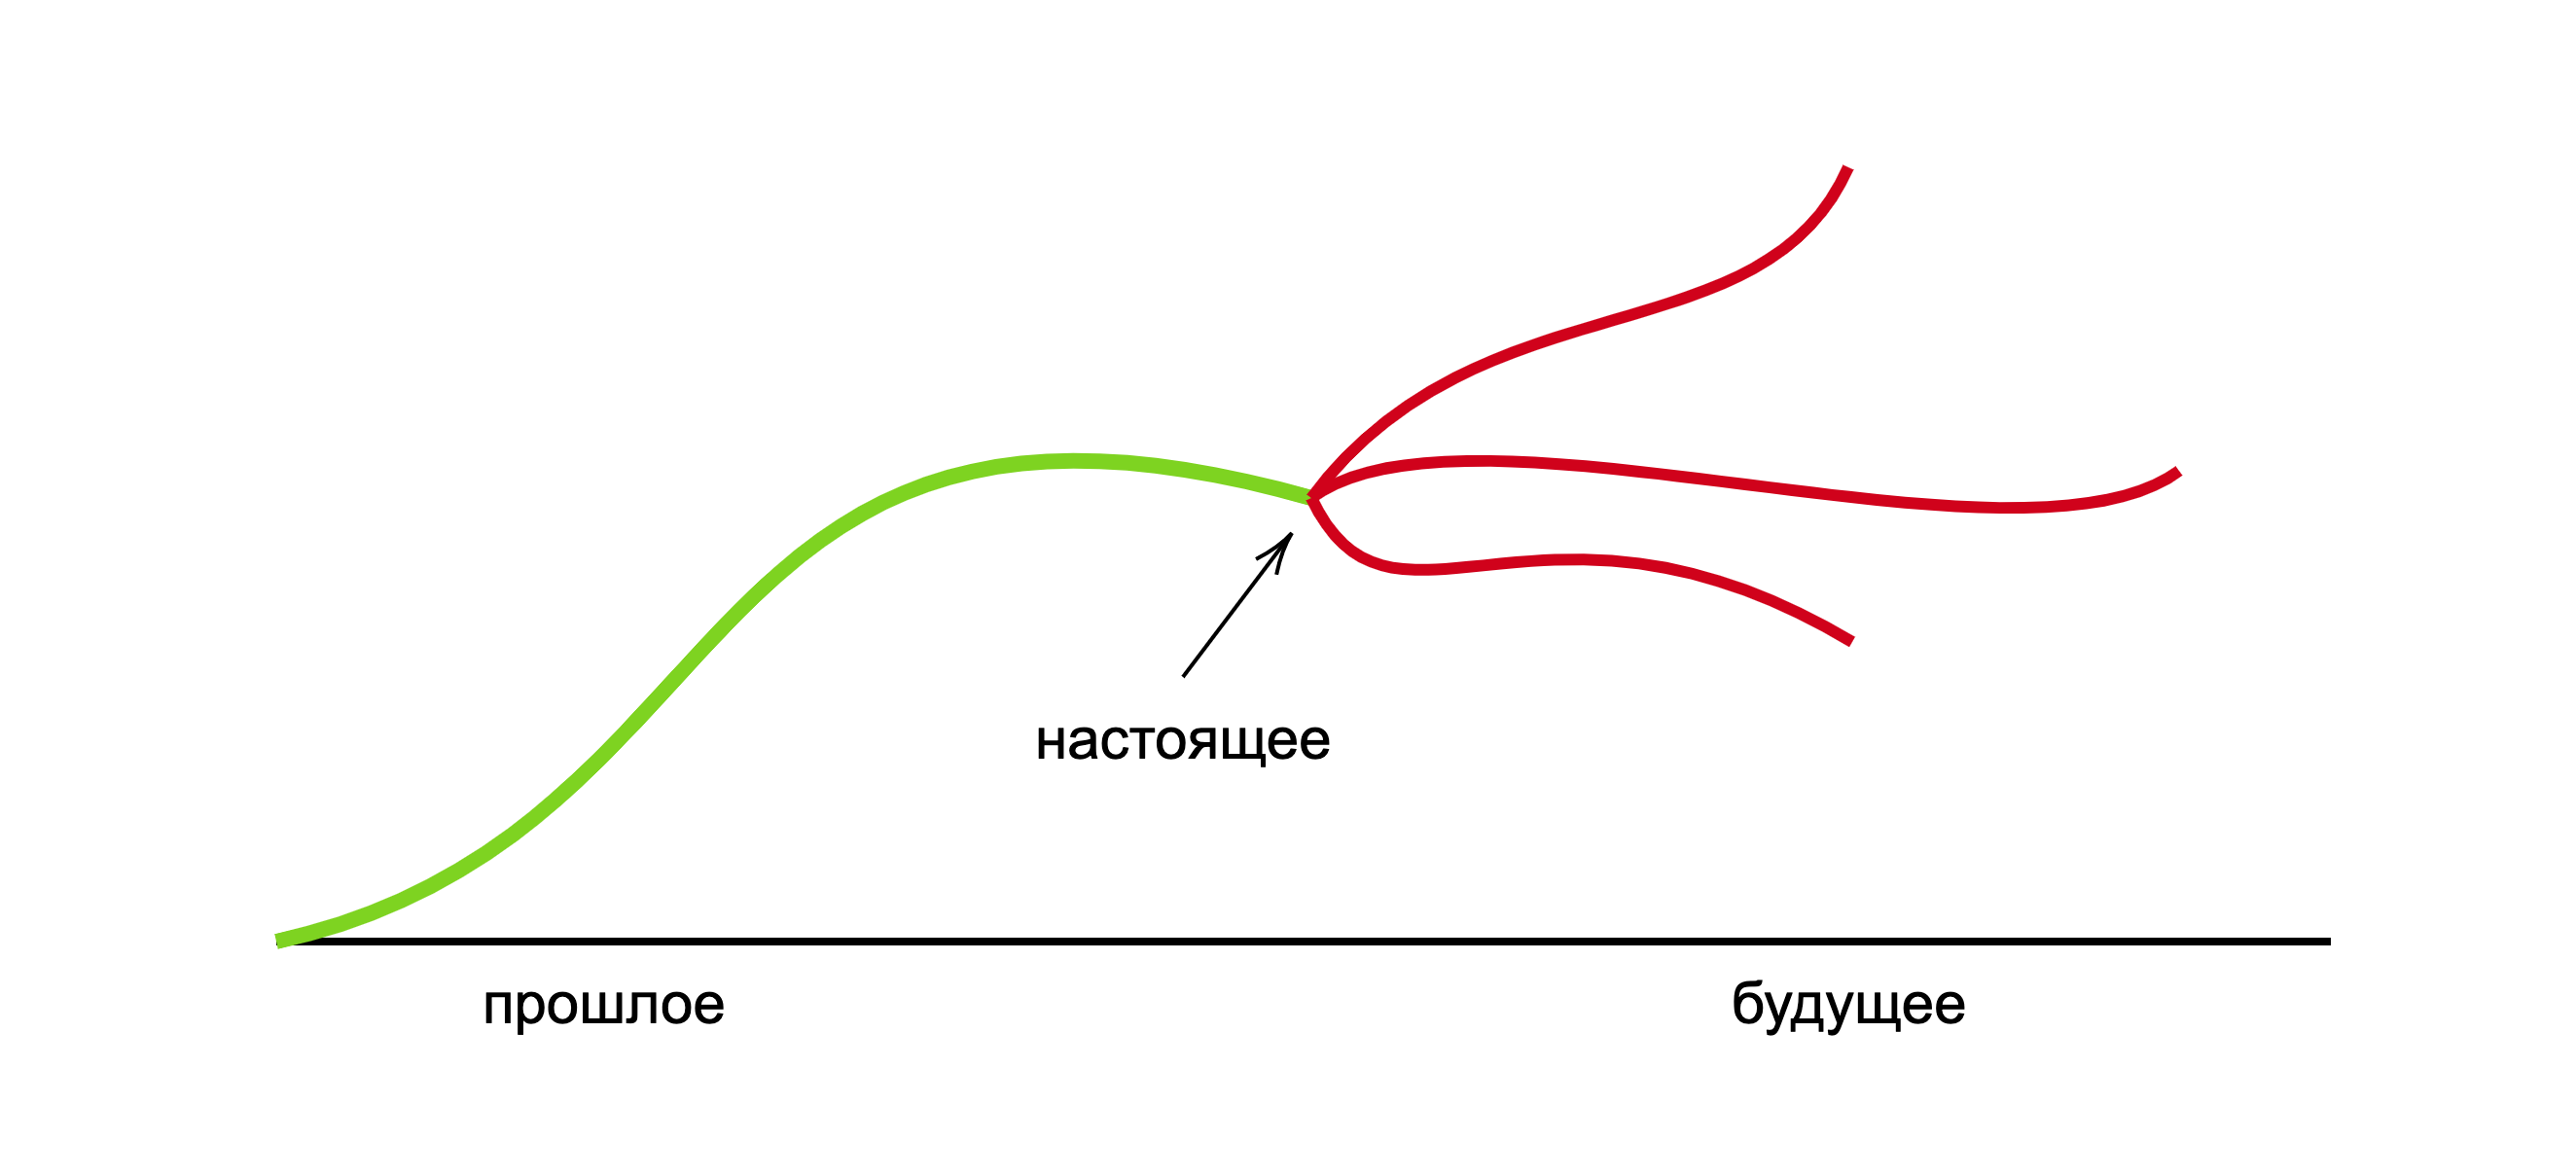
\includegraphics[width=1.0\textwidth]{img/pred_task_diagram_t.png}
	\caption{Иллюстрация прогноза по времени в задачах прогнозирования}
	\label{fig:components}
\end{figure}

Виды задач прогнозирования:
\begin{itemize}
	
	\item[---] Биржевая торговля: прогнозирование котировок и индексов на бирже.
	\item[---] Управляющие системы: прогноз показателей работы электрогенераторов.
	\item[---] Экономика: прогнозирование стоимости недвижимости
	\item[---] Демография: прогноз изменения численности населения конкретных социальных групп в заданной локации
	\item[---] Гидрометеорология: прогнозирование вулканической активности
	
\end{itemize}

\subsection{Постановка задачи}

В рассматриваемой задаче цель состоит в том, чтобы предсказать оставшийся полезный срок службы (RUL --- {\it Remaining Useful Life}) каждого двигателя в наборе тестовых данных. RUL эквивалентно количеству полетов, оставшихся до отказа двигателя после последней точки данных в тестовом наборе данных.

\subsubsection{Описание эксперимента}

Наборы данных состоят из 26 временных рядов. Данные представляют собой показания датчиков в двигателях. Каждый набор данных далее делится на обучающие и тестовые выборки. Каждый временной ряд относится к определенному отдельно взятому двигателю, т. е. можно считать, что данные относятся к парку двигателей одного и того же типа. Каждый двигатель запускается с разной степенью начального износа и производственными отклонениями, которые неизвестны системе. Этот износ и отклонения считаются нормальными, т. е. не считаются дефектом или неисправностью. Есть три рабочих режима (в наборе данных указано, как {\it operational setting}), которые существенно влияют на работу двигателя, однако их описания отсутствуют.  Эти настройки также включены в данные. Обучение производится на 80\% обучающей выборки. Остальные 20\% данных в обучающей выборке отложены для валидации модели. Данные загрязнены шумом датчиков.

Двигатель работает должным образом в начале каждого временного ряда и в какой-то момент времени выдает неисправность. В обучающей выборке неисправность нарастает до отказа системы. В тестовом наборе данных временной ряд заканчивается за некоторое время $t$ до сбоя системы. Цель задачи --- спрогнозировать количество оставшихся рабочих циклов до отказа в испытательной установке, то есть количество рабочих циклов после последнего текущего цикла, в которых двигатель будет продолжать работать. Также предоставлен вектор истинных значений оставшегося полезного срока службы (RUL), дабы сверить предсказанные и истинные значения и провести последующий анализ модели. 

\subsubsection{Описание набора данных}

Данные содержат 26 столбцов, содержащих числа, разделенные пробелами. Каждая строка представляет собой массив данных, снятых в течение одного рабочего цикла, каждый столбец --- это отдельная переменная.
\\
\\
Колонки содержат:
\begin{enumerate} 
	\item unit number --- номер двигателя
	\item time, in cycles --- время в циклах
	\item operational setting 1 --- режим полёта 1
	\item operational setting 2 --- режим полёта 2
	\item operational setting 3 --- режим полёта 3
	\item sensor measurement 1 --- измерение датчика 1	
	\item sensor measurement 2 --- измерение датчика 2
	\\
	...
	\setcounter{enumi}{25}
	\item sensor measurement 26 --- измерение датчика 26
\end{enumerate}

\subsection{Сведение к задаче глубинного обучения} 

Традиционные подходы к решению задач прогнозирования временных рядов включают в себя регрессионные модели прогнозирования, авторегрессионные модели прогнозирования (ARIMAX, GARCH, ARDLM), модели по выборке максимального подобия (MMSP), модели на основе генетического алгоритма (GA) и множество других.

В последние годы развитие в области искусственного интеллекта и глубинного обучения привело к тому, что новые алгоритмы на основе нейронных сетей в разы превосходят уже существующие традиционные подходы к решению широкого спектра задач \cite{Sholtanyuk}. И одним из таких алгоритмов является модель LSTM --- особый вид RNN, способный запоминать долгосрочные зависимости. 

\section{LSTM}

\subsection{Проблема долговременных зависимостей}

Одним из преимуществ рекуррентных нейронных сетей (RNN) является то, что они способны сохранять сжатую историческую информацию из предыдущих слоёв сети и подавать её на вход текущему слою, что в свою очередь существенно повышает качество используемой модели.

\begin{figure}[h]
	\centering
	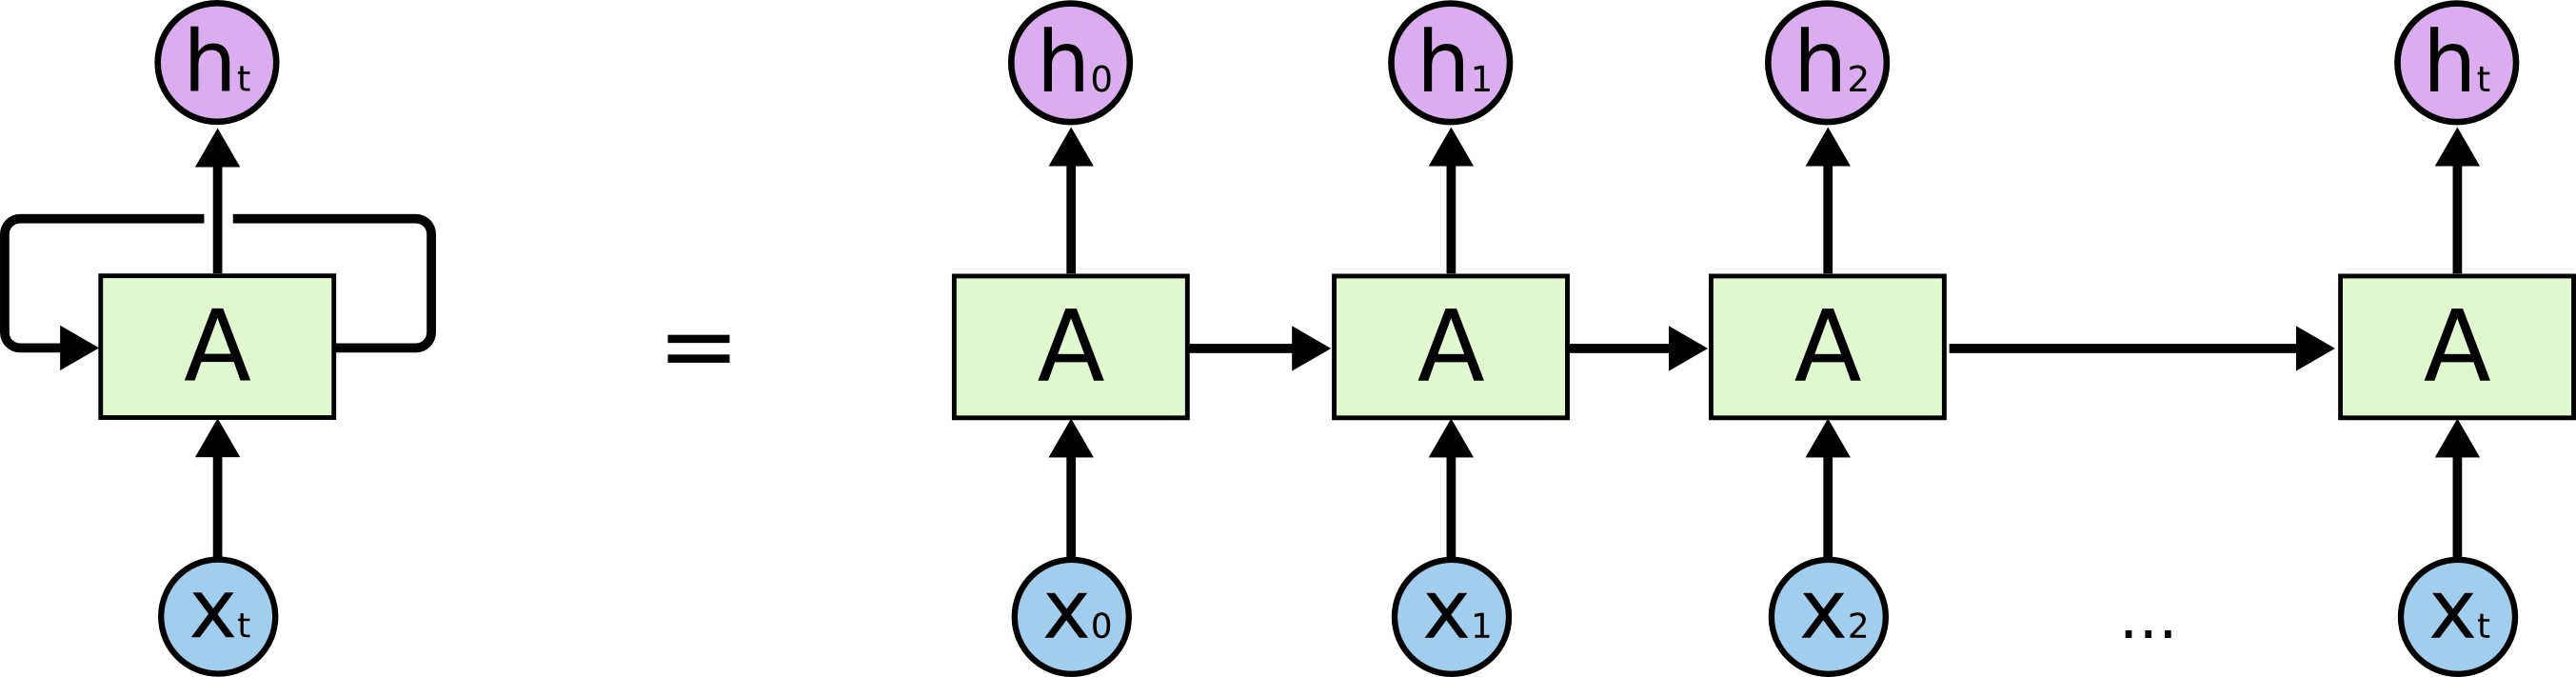
\includegraphics[width=0.85\textwidth]{img/RNN-unrolled.png}
	\caption{Развёрнутое представление рекуррентной нейронной сети. Взято из \cite{Colah}}
	\label{fig:rnn}
\end{figure}

На приведенной выше схеме небольшая часть нейронной сети $A$, на вход которой подается некоторый вектор $x_t$ и на выходе извлекатеся вектор скрытого состояния $h_t$. Таким образом рекуррентную нейронную сеть можно рассматривать как несколько копий одной и той же сети, каждая из которых, в свою очередь, передает сообщение своему преемнику на следующий шаг. Это демонстрирует, что рекуррентные нейронные сети тесно связаны с последовательностями и списками, что отлично подходит для работы с данными таких типов. 

Бывают случаи, когда для выполнения какой-либо задачи нам требуется только “недавняя” информация. К примеру, это справедливо в случае, когда рассмотривается языковая модель, которая пытается предсказать следующее слово в предложении. Если нам хочется предсказывать последнее слово в предложении “автобус прибывает на вокзал”, достаточно контекста длинною в пару слов с обеих сторон интересующего нас слова. В этом случае понятно, что последним словом будет “вокзал”. Отсюда очевидно, что когда расстояние между актуальной информацией и позицией, где она понадобилась, небольшое, рекуррентные нейронные сети могут обучиться довольно хорошо, используя лишь информацию из нескольких предыдущих слоёв.

Но бывает так, что для корректной работы требуется больше контекста. Рассмотрим случай, когда нам хочется предсказывать последнее слово в тексте “В детстве я жил в Италии <текст> Я едва-ли знаю итальянский”. Ближайший контекст намекает на то, что последним словом должен быть язык, но чтобы понять, какой именно язык, нам необходим больший контекст, упоминающий Италию в более далёком прошлом. Таким образом, расстояние между текущей информацией и позицией её применения может стать очень большим. К несчатью, с ростом этого расстояния, рекуррентные нейронные сети теряют способность связывать информацию такого вида.

Если углубиться в рекуррентные нейронные сети, то с теоретической точки зрения проблем с обработкой долговременных зависимостей у RNN быть не должно. Можно тщательно настраивать и подбирать параметры сети для решения задач различных видов. Но на практике обучить сеть такого рода параметрам кажется невыполнимой задачей. Над этой проблемой усердно работала команда Йошуа Бенджио (Yoshua Bengio), 1994 \cite{Bengio}. Они показали, что на практике действительно невозможно разрешить данную задачу.

\subsection{LSTM сеть}

Долгая краткосрочная память (Long short-term memory; LSTM) --- это особый вид архитектуры рекуррентных нейронных сетей, которая способна к обучению долговременным зависимостям. Такого рода сети были впервые представлены в работе Хохрайтера и Шмидхубера в 1997 \cite{Hochreiter} году, а затем были неоднократно доработаны и усовершенствованы в работах множества других исследователей в области искуственного интеллекта и машинного обучения. LSTM-сети отлично подходят для целого ряда разнообразных задач и в настоящее время являются неплохой базой для построения моделей в области обработки естественного языка.

LSTM-архитектура создавалась специально для решения проблемы долговременных зависимостей, присущей классическим RNN. Главным свойством таких сетей является запоминание и хранение контекста большой длинны. Классическая RNN-подобная нейронная сеть имеет форму последовательности одинаковых повторяющихся слоёв. В обычной рекуррентной нейронной сети строение одного такого модуля очень простое. К примеру, такой модуль может представлять собой один слой с функцией активации типа сигмоида (график [\ref{fig:sigmoid}]) или гиперболический тангенс.

\begin{figure}[h]
	\centering
	\includegraphics[width=0.8\textwidth]{img/sigmoid.png}
	\caption{График функции Sigmoid. Взято из \cite{Sigmoid-Wiki}}
	\label{fig:sigmoid}
\end{figure}


Аналогично классической RNN, LSTM-структура также представляет собой последовательность, но имеет совершенно другие внутренние слои. Вместо одного слоя нейронной сети у LSTM их четыре, к тому же взаимодействие между ними происходит совершенно иным образом. 

\begin{figure}[h]
	\centering
	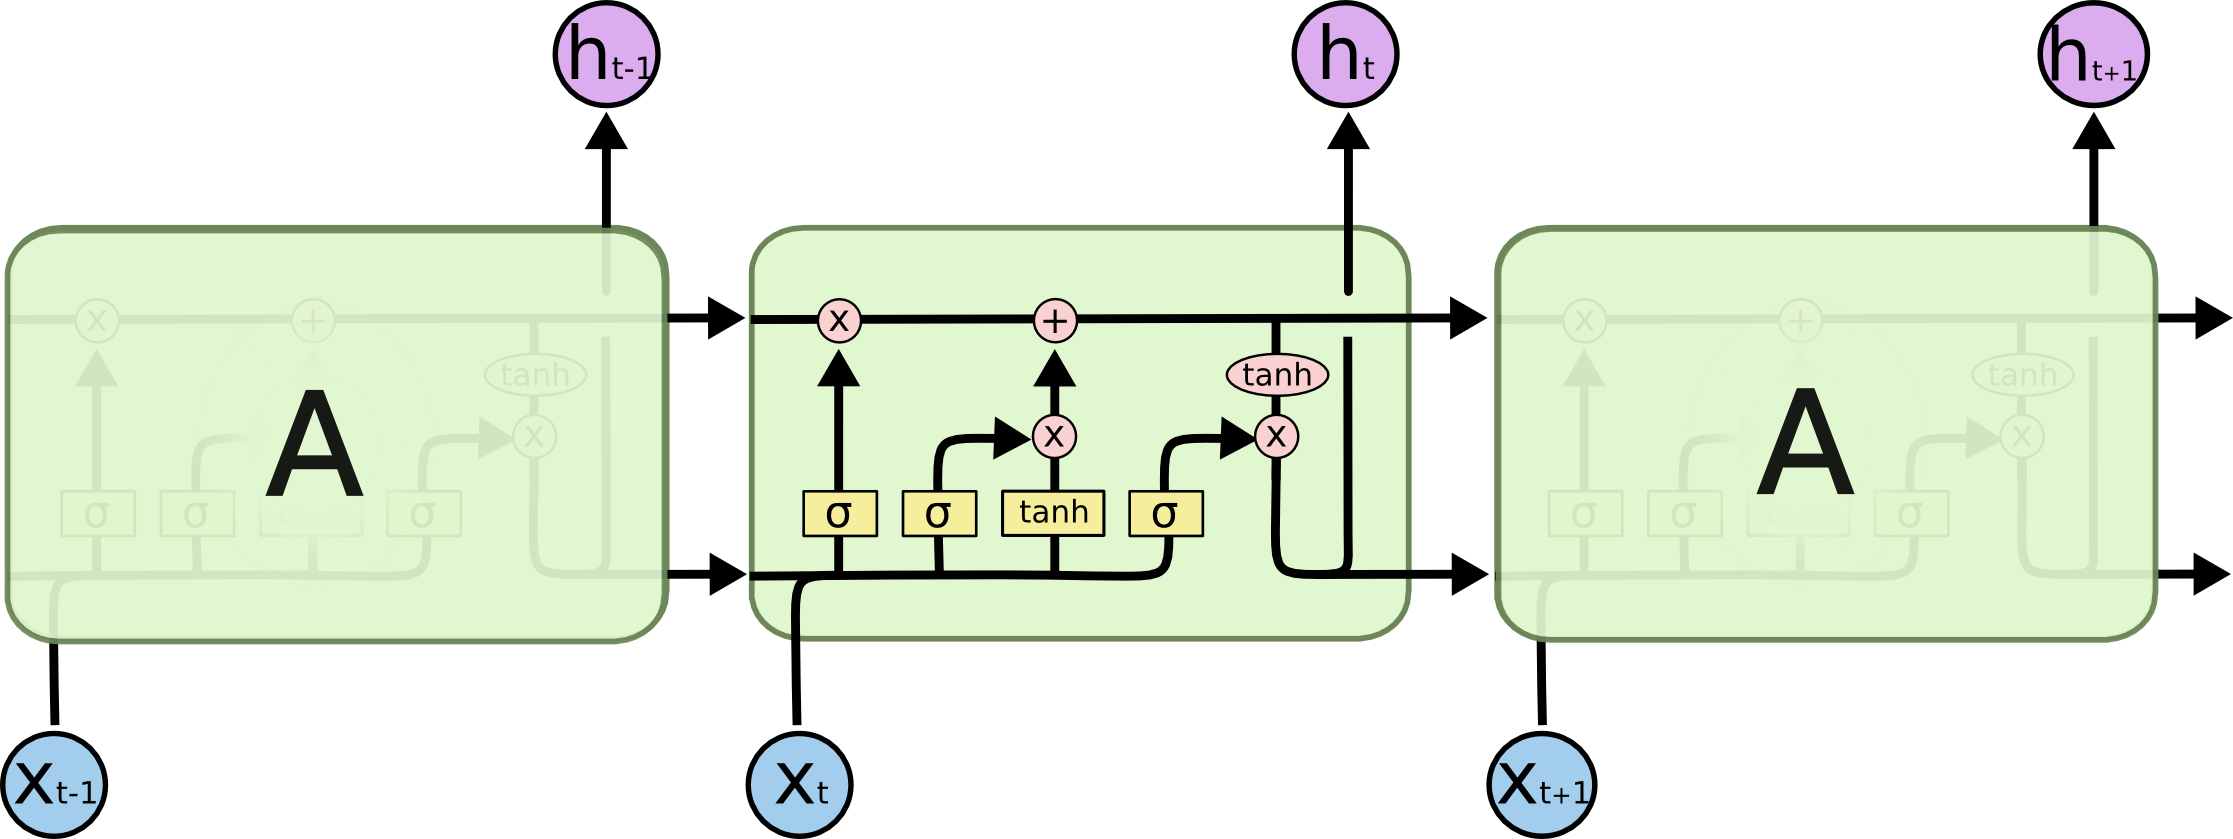
\includegraphics[width=1\textwidth]{img/LSTM-chain.png}
	\caption{Модуль LSTM содержит четыре слоя. Взято из \cite{Colah}}
	\label{fig:lstm}
\end{figure}

На схеме [\ref{fig:lstm}] каждая стрелка переносит вектор от выхода одного модуля и подаёт его на вход следующего. Красными кругами обозначены поэлементные операции, такие, как сложение или перемножение векторов. Жёлтые прямоугольники соответствуют слоям нейронной сети. Сходящиеся стрелки означают объединение, а разветвляющиеся стрелки отвечают за копирование данных и их передачу в другие компоненты сети.

Главная концепция LSTM --- состояние ячейки ({\it cell state}) --- это горизонтальная линия, проходящая по верхней части схемы. Состояние ячейки проходит напрямую через всю последовательность, участвуя лишь в нескольких линейных преобразованиях. Информация может легко "протекать" по ней, не подвергаясь никаким изменениям. Также LSTM может стирать информацию из внутреннего состояния ячейки. Этот процесс регулируется так называемыми фильтрами ({\it gates}). На основании некоторых условий фильтры способны пропускать информацию. Они состоят из слоя сигмоидальной нейронной сети и операции поэлементного умножения. Сигмоидальный слой возвращает числа от нуля до единицы, которые обозначают, какую долю каждого блока информации следует пропустить дальше по сети. Ноль в данном случае означает “не пропускать ничего”, единица --- “пропустить все”. LSTM имеет три таких фильтра, позволяющих защищать и контролировать состояние ячейки.


\subsection{Шаги работы}

\begin{enumerate}

\item
Первый шаг работы LSTM --- определить ненужную информацию в состоянии ячейки и избавиться от неё. Этим занимается слой сигмоиды, называемый «слоем фильтра забывания» (forget gate layer). Такой слой смотрит на $h_{t-1}$  и $x_t$ и возвращает значение от 0 до 1 для каждого числа из состояния ячейки $C_{t-1}$. Единица означает «полностью сохранить», а ноль – «полностью выбросить».

\begin{figure}[h]
	\centering
	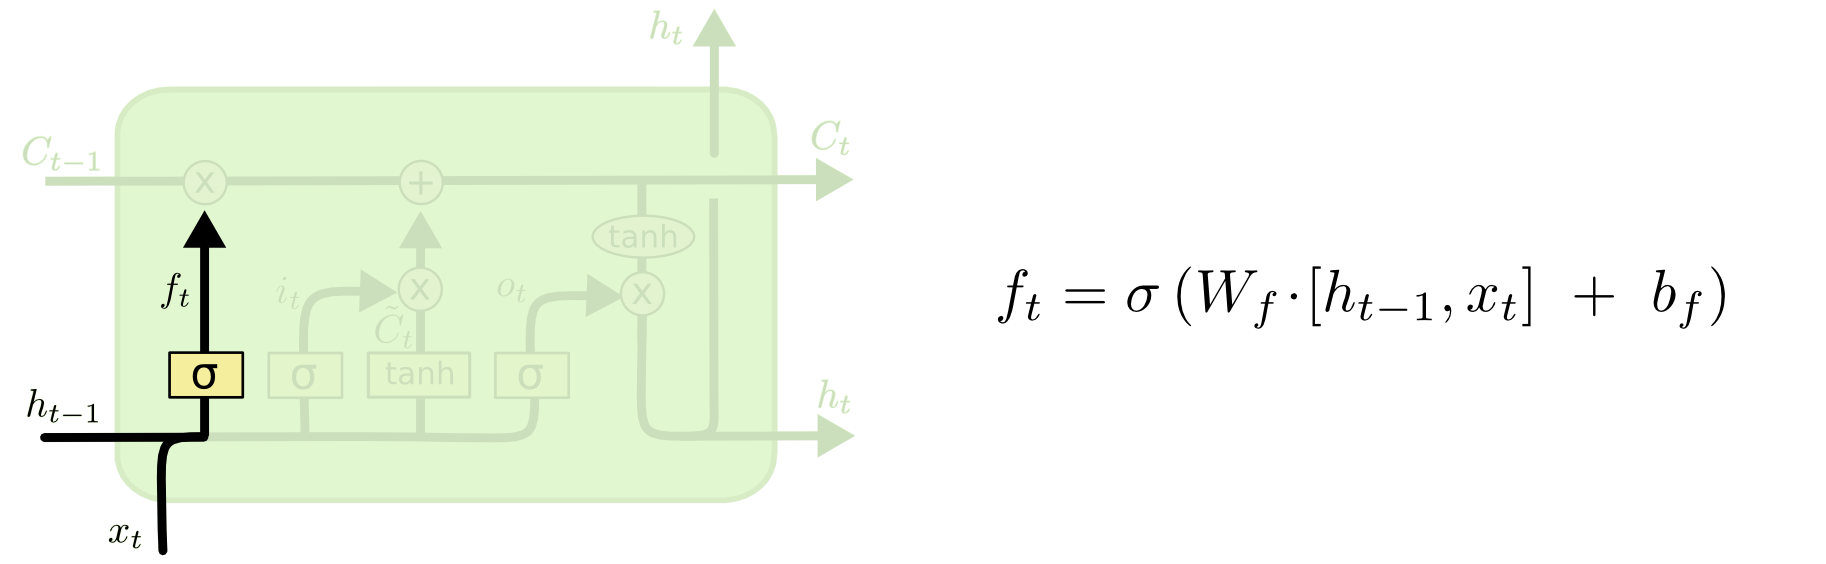
\includegraphics[width=1\textwidth]{img/LSTM-step_1.png}
	\caption{Первый шаг. Взято из \cite{Colah}}
	\label{fig:lstm-s1}
\end{figure}

\item
На следующем шаге требуется определить, какая именно новая информация будет храниться в состоянии ячейки. Сперва {\it input layer gate}, или {\it слой входного фильтра} определяет, какие значения следует обновить. Потом tanh-слой строит вектор новых значений-кандидатов $\widetilde{C_t}$, которые возможно добавить в состояние ячейки.

\begin{figure}[h]
	\centering
	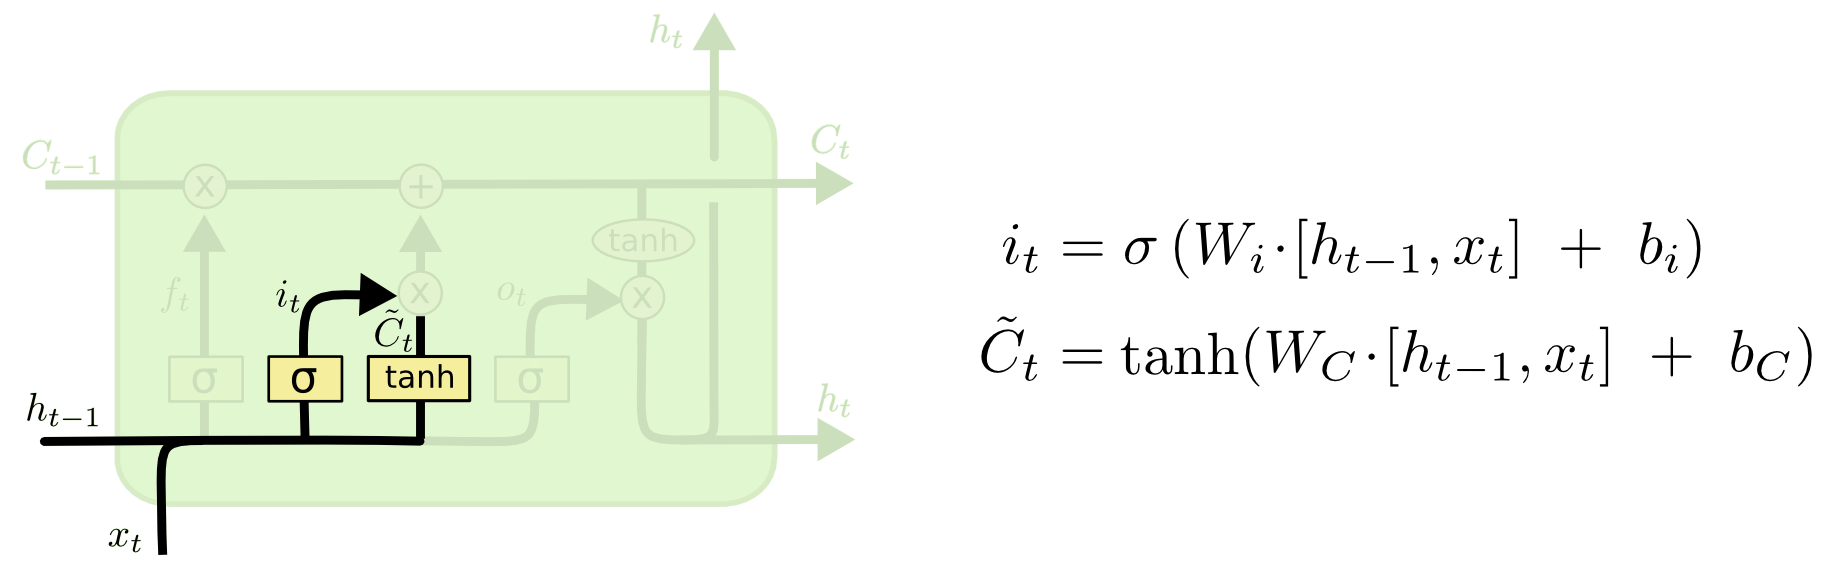
\includegraphics[width=1\textwidth]{img/LSTM_step_2.png}
	\caption{Второй шаг. Взято из \cite{Colah}}
	\label{fig:lstm-s2}
\end{figure}

\item
Следующим шагом требуется заменить старое состояние ячейки $C_{t - 1}$  на новое $C_t$. Для этого нужно умножить старое состояние на $f_t$, тем самым как-бы забывая ненужную информацию. Затем прибавляется $i_t * \widetilde{C_t}$, чтобы получить информацию о том, на какую величину нужно обновить каждое из значений нового состояния.

\begin{figure}[h]
	\centering
	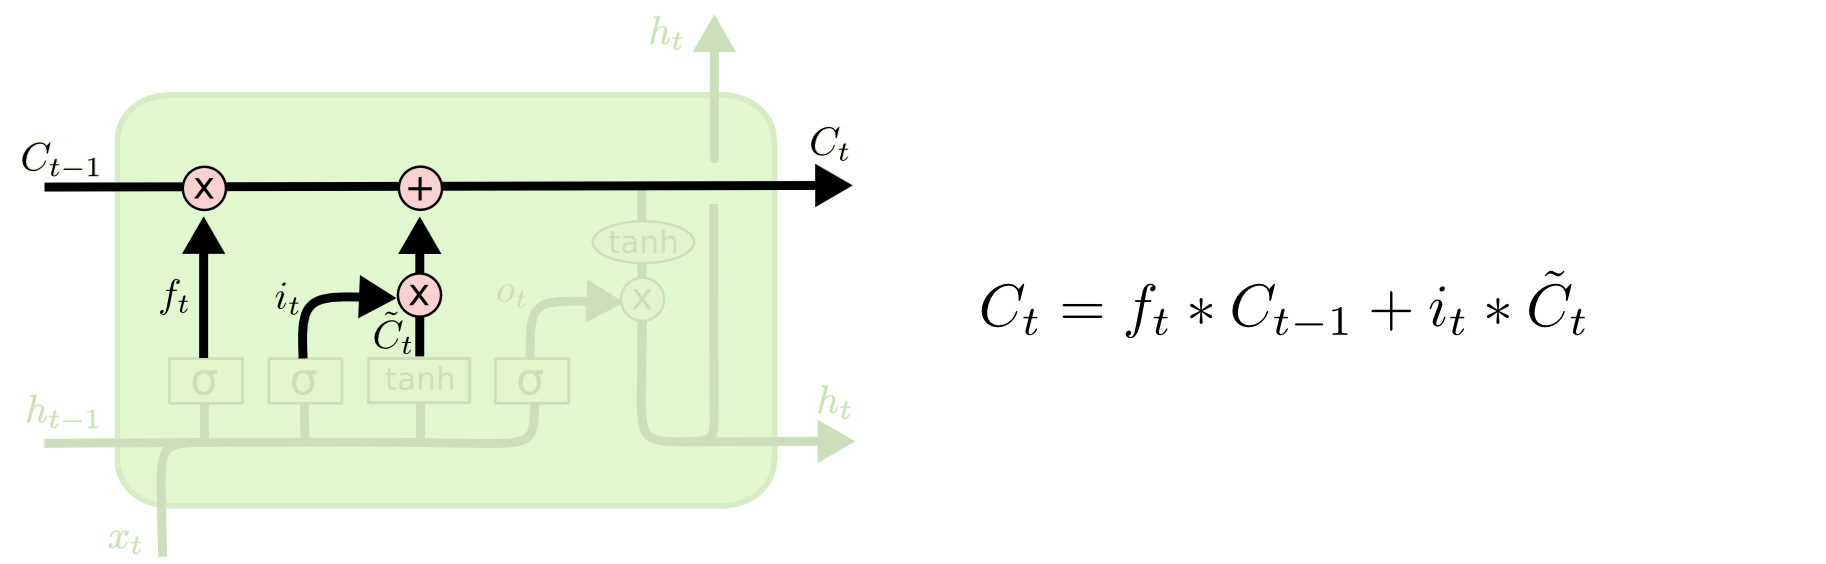
\includegraphics[width=1\textwidth]{img/LSTM_step_3.png}
	\caption{Третий шаг. Взято из \cite{Colah}}
	\label{fig:lstm-s3}
\end{figure}

\item
На последнем шаге нужно решить, какая информация должна быть на выходе. Выходные данные будут основаны на текущем состоянии ячейки. Сначала требуется применить слой сигмоиды, который определяет, какую информацию из состояния ячейки мы будем выводить. Затем применяется tanh-слой, чтобы получить на выходе значения из диапазона от -1 до 1, которые перемножаются с выходными значениями слоя сигмоиды, что позволяет выводить только требуемую информацию.

\begin{figure}[h]
	\centering
	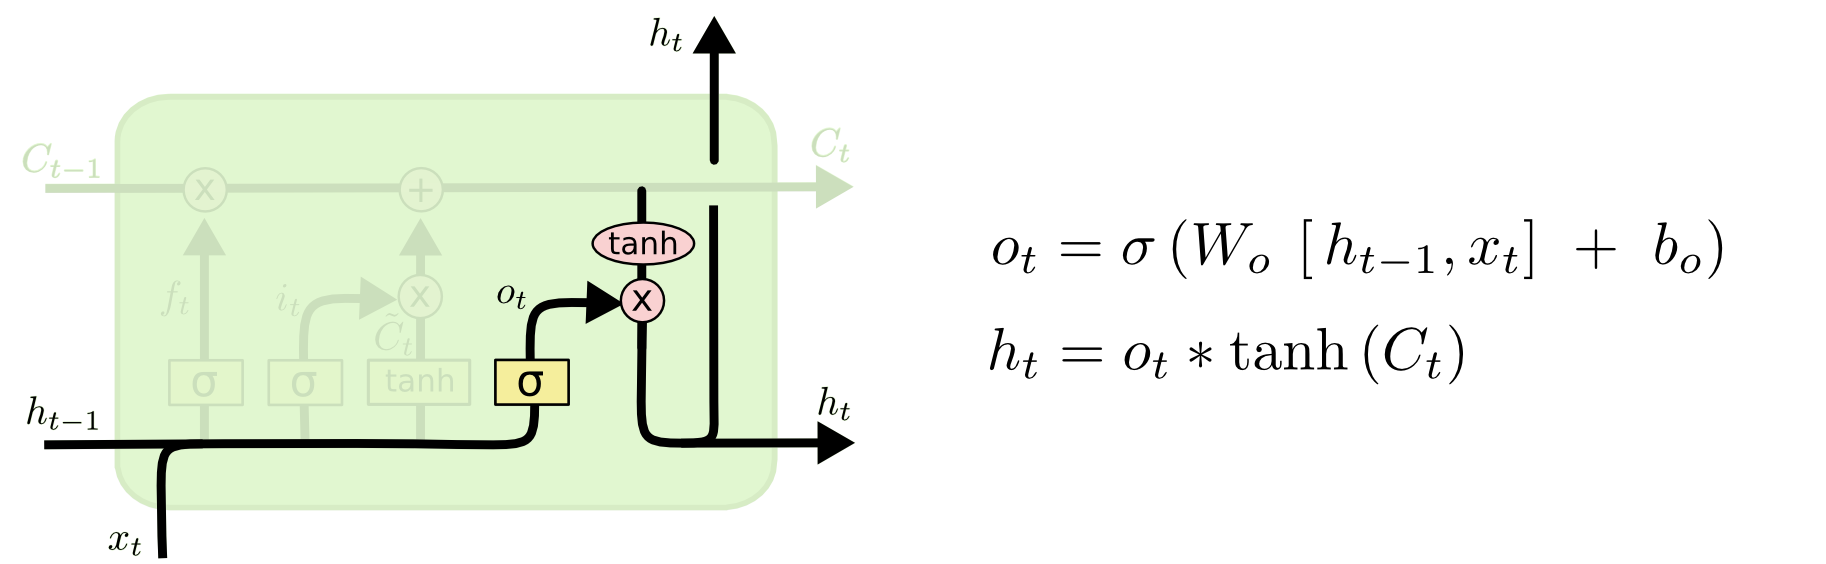
\includegraphics[width=1\textwidth]{img/LSTM_step_4.png}
	\caption{Четвёртый шаг. Взято из \cite{Colah}}
	\label{fig:lstm-s4}
\end{figure}

\end{enumerate}

\newpage

\section{Вычислительный эксперимент}

\subsection{Предобработка данных}

Для экспериментов был выбран набор данных с сайта NASA за авторством A. Saxena, K. Goebel, D. Simon, and N. Eklund (2008) \cite{Saxena}, содержащий:

\begin{itemize}
    \item $\sim$20,000 паттернов в обучающей выборке, 100 уникальных идентификаторов двигателей;
    \item $\sim$13,000 строк в тестовой выборке, 100 уникальных идентификаторов двигателей;
    \item 100 строк --- истинные значения
\end{itemize}

Из данных были удалены попарно скореллированные признаки (> 80\% корелляции), как из обучающей выборки, так и из тестовой выборки. Далее, оба набора данных были очищены от шума, пробелы в колонках были заменены на усреднённые показания по конкретно рассматриваемому признаку. Также была произведена нормировка признаков с помощью MinMaxScaler:

% \begin{equation}
$$x_{scaled} = \frac{x - x_{min}}{x_{max} - x_{min}}$$ 
% \end{equation}



\subsection{Обучение модели}

В качестве модели используется глубокуя LSTM сеть. На первом слое --- LSTM со 100 единицами ({\it units --- размерность выходного пространства}), за которым следует еще один слой LSTM с 50 единицами. \hyperref[glossary]{Dropout}, равный $0.2$ применяется после каждого слоя LSTM для улучшения точности модели, а также во избежание переобучения. Последний слой --- это полносвязная сеть с активацией типа сигмоида и одномерным выходом. Архитектура нейронной сети представлена на схеме \ref{table_1}:

\begin{table}[h]
	\large
	\centering
	\begin{tabular}{p{0.4\linewidth}p{0.3\linewidth}p{0.2\linewidth}}
		\multicolumn{3}{p{0.9\linewidth}}{{\bf Модель: sequential\_1}} \\
		\hline
		Слой (тип) & Размерность выхода & Кол-во параметров \\
		\hline
		\hline
		lstm\_1 (LSTM) & (50, 100) & 50400 \\
		\hline
		dropout\_1 (Dropout) & (50, 100) & 0 \\
		\hline
		lstm\_2 (LSTM) & (50) & 30,200 \\
		\hline
		dropout\_2 (Dropout) & (50) & 0 \\
		\hline
		dense\_1 (Dense) & (1) & 51 \\
		\hline
		activation\_1 (Activation) & (1) & 0 \\
		\hline
		\hline
		\multicolumn{3}{p{0.9\linewidth}}{{\bf Всего параметров: 80,651}} \\[-3mm]
		\multicolumn{3}{p{0.9\linewidth}}{{\bf Обучаемых параметров: 80,651}} \\
	\end{tabular}
	\caption{Архитектура сети}
	\label{table_1}
\end{table}

Дополнительно, используется механизм Early Stopping --- остановка обучения нейронной сети при выходе ошибки на плато либо при её систематическом увеличении для избежания ухудшения параметров сети. Сеть обучается на протяжении 100 эпох ({\it epoch} --- полный цикл обучения). Размер батча ({\it batch --- кусок данных для обучения на конкретном шаге}) равен 200. В качестве метрик используются $MAE$ ({\it mean absolute error}) и коэффициент детерминации $R^2$  --- универсальная мера зависимости одной случайной величины от множества других. Все описанные параметры сети являются оптимальными и были получены эксперементальным путём в ходе процедуры \hyperref[glossary]{Grid Search}.

Ниже приведён алгоритм обучения модели:

\begin{algorithm}[H]
	\caption{{Процедура обучения}}
	
	\begin{algorithmic}[1]
		\STATE Разбить обучающую выборку на батчи $X_{batch} = \{\textbf{x}[i]\}_{i = 1}^{n}$ по 200 элементов
		\FOR{$\text{t}=1,\dots num\_epochs$}
		\STATE Подать на вход последовательность из батча в виде вектора
		\STATE Вычислить предсказание на текущем шаге
		\STATE Сделать шаг градиентной оптимизации
		\STATE Если ошибка при валидации на текущем шаге больше, чем при последней проверке --- остановить обучение и сохранить параметры сети
		\STATE Перейти на следующую итерацию
		\ENDFOR
		
		\hspace*{\algorithmicindent} \textbf{Выход:} усреднённые значения остаточного числа циклов работы двигателя за $n$ батчей
	\end{algorithmic}
\end{algorithm}

\subsection{Валидация модели}

Так как рассматриваемые данные представляют собой временные ряды, то очень важную роль играет их временная структура, а следовательно, в отличие от случайных выборок, они могут содержать в себе дополнительную важную для обучения информацию, которую нельзя терять. Поэтому стандартные техники валидации в этом случае являются непригодными для использования. Таким образом, в процессе валидации пришлось использовать более специфический способ для оптимизации параметров, так называемый {\it cross-validation on a rolling basis} или кросс-валидация c использованием скользящего окна. 

\begin{figure}[h]
	\centering
	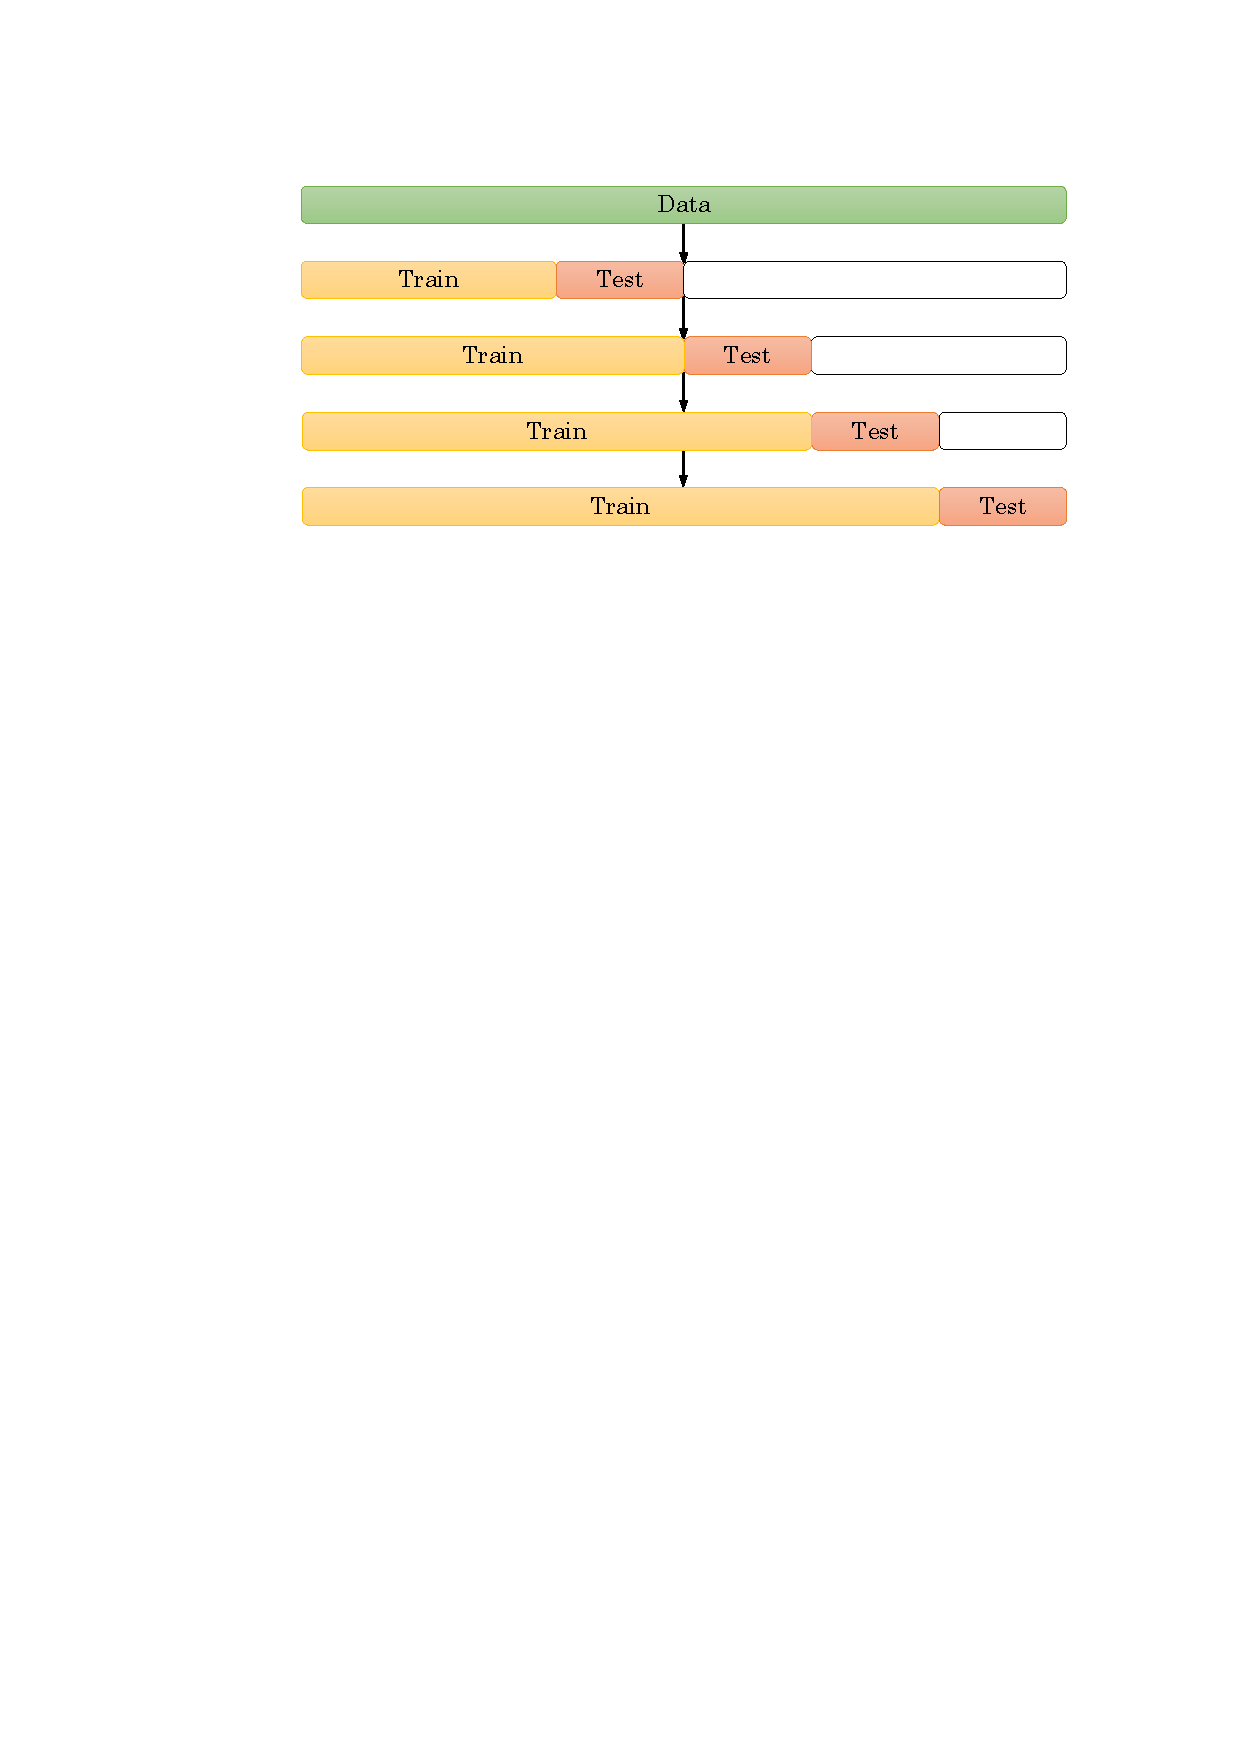
\includegraphics[width=0.95\textwidth]{img/sliding_window_val.pdf}
	\caption{Схема валидации}
	\label{fig:sliding_window}
\end{figure}

Принцип этого подхода состоит в том, что изначально модель начинает обучаться на небольшом отрезке временного ряда, с самого начала до конкретного момента времени $t$. Потом делается предсказание на $t + n$  шагов вперед и вычисляется ошибка. Далее обучающая выборка расширяется до значения $t + n$ и прогнозируется с $t + n$ до $t + 2n$. Так продолжает двигаться валидационный отрезок ряда до тех пор, пока не упирается в последнее доступное наблюдение. В итоге получится столько фолдов --- групп данных, сколько $n$ поместится в промежуток между изначальным обучающим отрезком и всей длиной рассматриваемого ряда.


\subsection{Результаты}

Обученная модель проверялась на тестовой выборке. Как и при обучении, одной из метрик выбиралась $MAE$. Для итогового теста использовались наилучшие параметры сети, выбранные эксперементальным путём в процессе обучения. Ниже на графиках представлены кривые данных метрик полученные при обучении и тестировании модели. Зелёный цвет отвечает за обучающую выборку, синий --- за тестовую.

На графике зависимости ошибки $MAE$ от количества циклов обучения [\ref{fig:test_mae}] видно, что примерно до 20-й эпохи ошибка стремительно падала, затем обучение начало замедляться и в какой-то момент вышло на плато. Начиная примерно с 25-й эпохи сеть вновь нашла оптимальное направление обновления градиента. Таким образом к 80-й итерации сеть сошлась к минимуму ошибки.

\begin{figure}
	\centering
	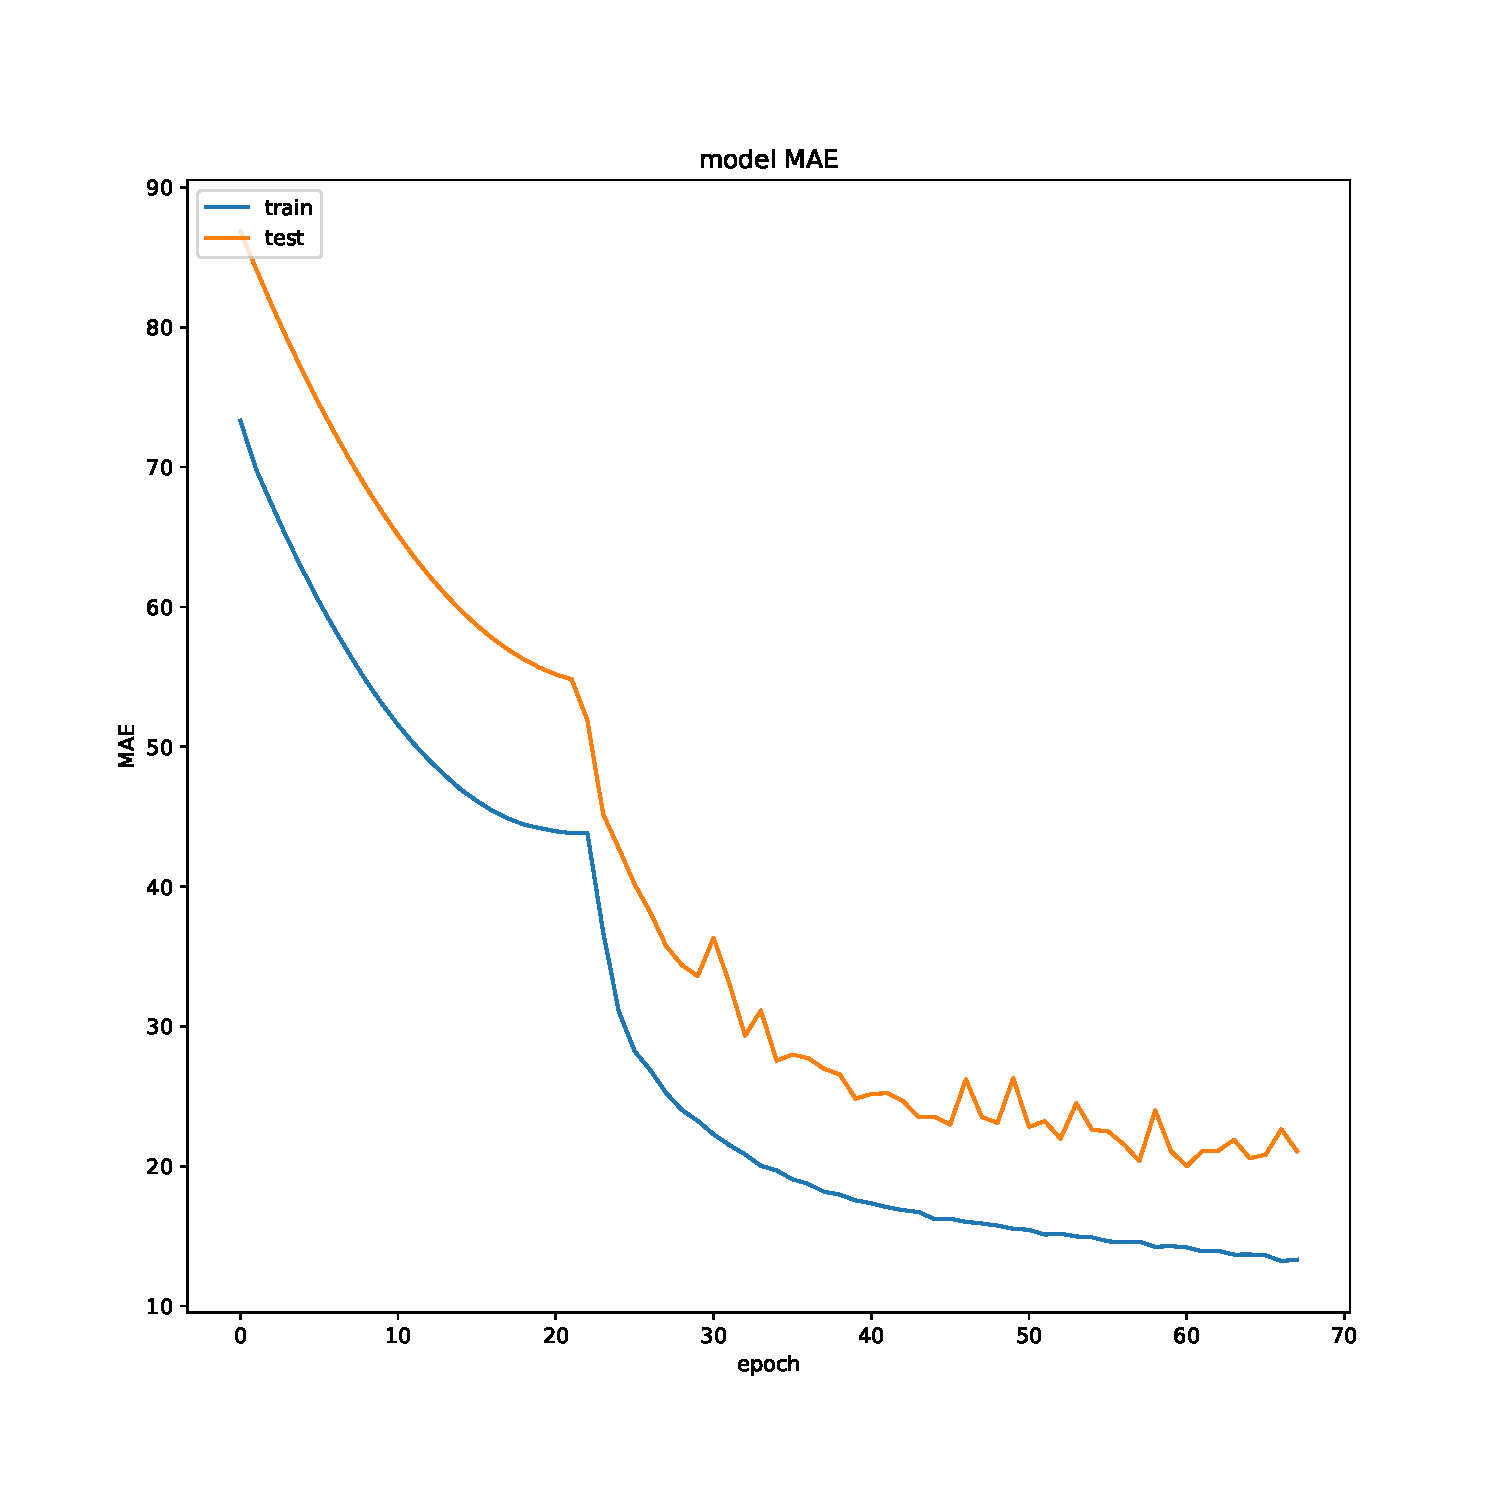
\includegraphics[width=0.9\textwidth]{img/model_mae.pdf}
	\caption{Кривые $MAE$}
	\label{fig:test_mae}
\end{figure}

\newpage

Также для итогового теста качества модели была использована метрика $R^2$ --- коэффициент детерминации. При оценке регрессионных моделей её можно трактовать, как соответствие модели данным или как долю дисперсии зависимой переменной, объясняемой моделью.

Из представленного графика [\ref{fig:test_r2}] видно, что коэффициент детерминации растёт в зависимости от количества циклов обучения модели. В случае обучающей выборки значение коэффициента $R^2$ достигает порога $\sim$0.86, что является показателем достаточно точного описания данных моделью, так как чем ближе коэффициент детерминации к значению 1, тем сильнее зависимость между данными и описывающим их алгоритмом-моделью. Как и в случае с $MAE$, из данного графика можно заметить, что на обучающей выборке коэффициент детерминации растёт более быстро и плавно, нежели на тестовой выборке.


\begin{figure}
	\centering
	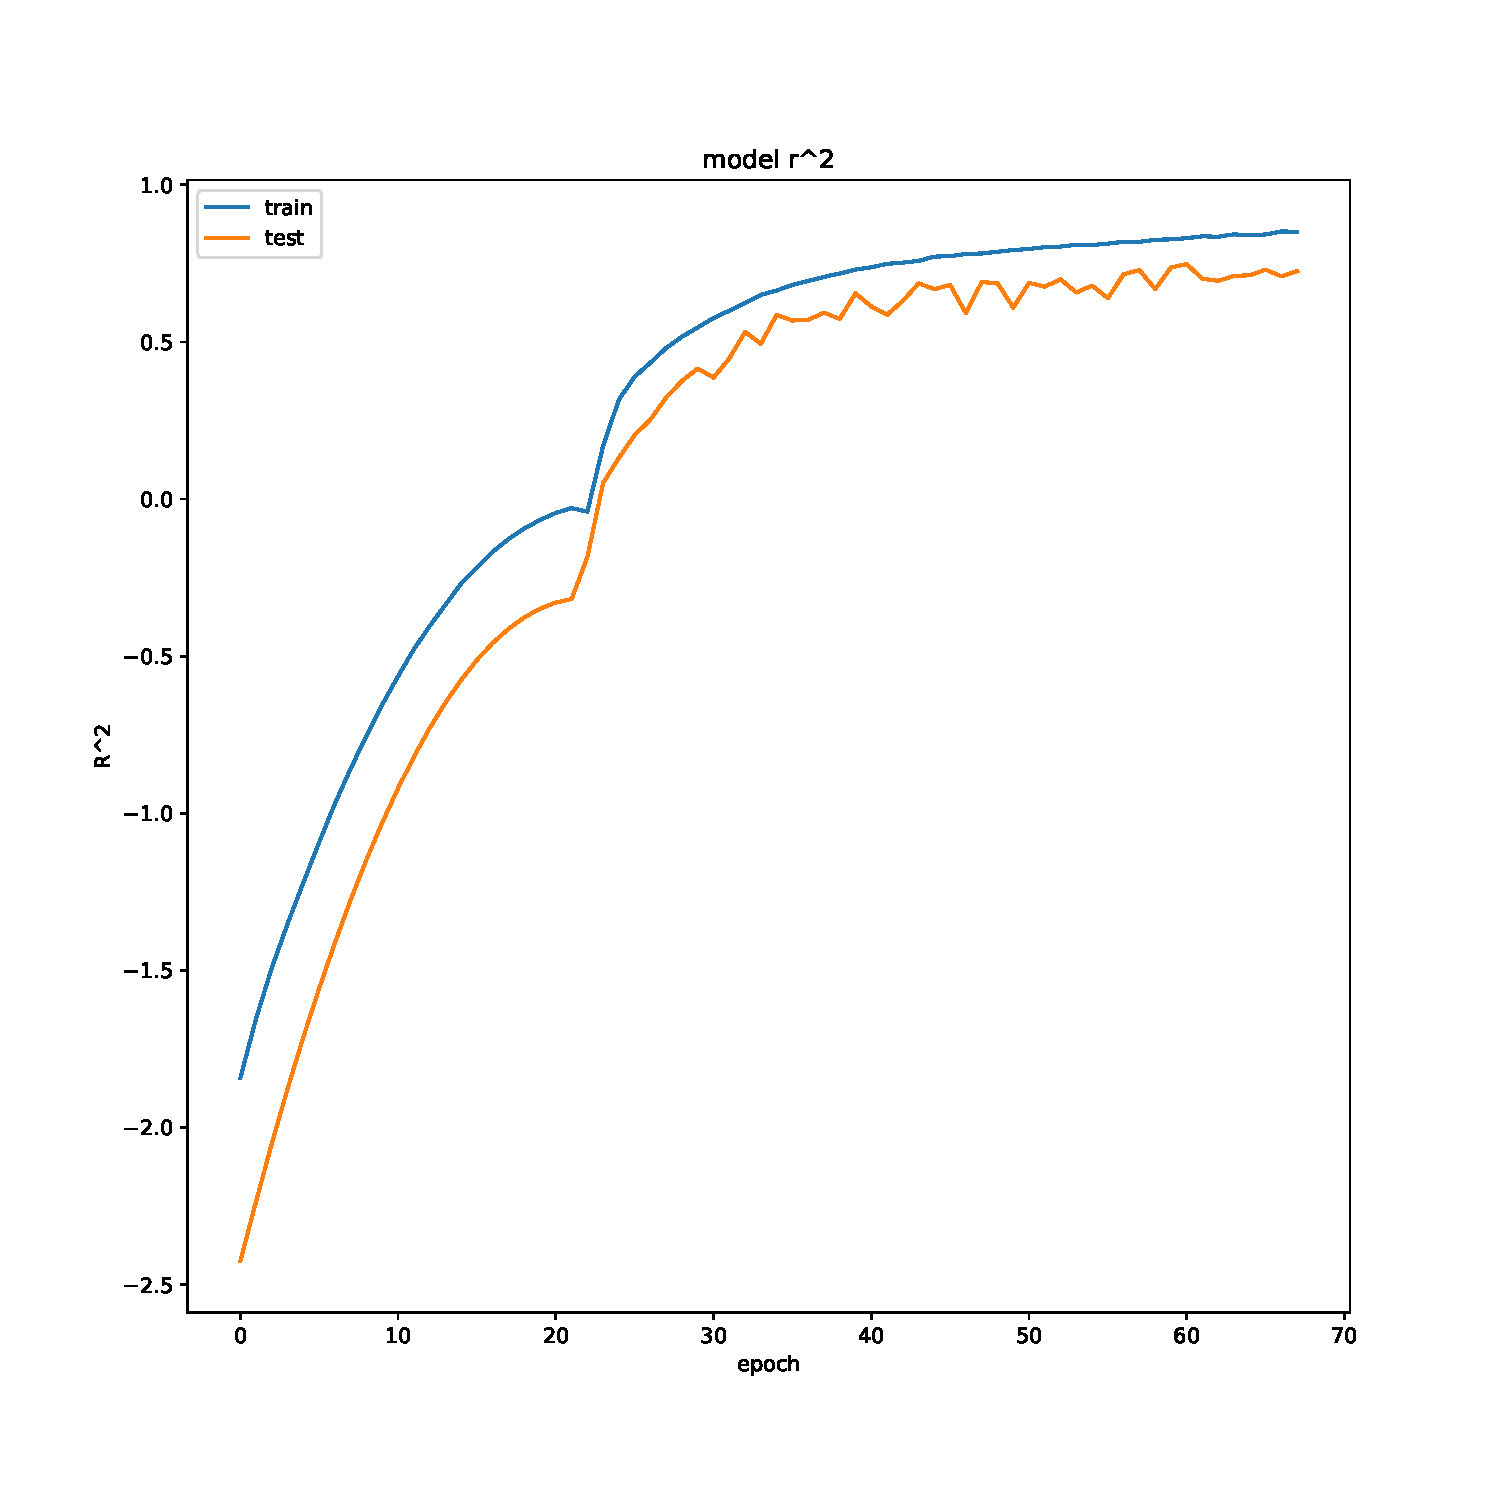
\includegraphics[width=0.9\textwidth]{img/model_r2.pdf}
	\caption{Кривые коэффициента детерминации $R^2$}
	\label{fig:test_r2}
\end{figure}

\newpage

Дополнительно был получен график, сравнивающий предсказанные значения на тестовой выборке с реальными \hyperref[glossary]{ground truth} метками. По оси абсцисс отображены 100 единиц двигателей, которые представлены в тестовой выборке. По оси ординат указано остаточное количество рабочих циклов для каждого двигателя. Синим цветом изображены истинные значения {\it RUL}, в то время как оранжевым обозначены предсказания, которые воспроизвела модель.

\begin{figure}[h]
	\centering
	\includegraphics[width=1\textwidth]{img/model_regression_1.pdf}
	\caption{Сравнение предсказанных меток с истинными для тестового набора данных}
	\label{fig:test_regression}
\end{figure}


\subsection{Сравнение со стандартными подходами}

\subsubsection{Random Forest}

Модель-алгоритм машинного обучения Random Forest ({\it случайный лес}) --- это множество решающих деревьев. В общем случае решающее дерево --- n-ичное дерево с решающими правилами в нелистовых узлах и некотором прогнозом по целевой функции в листовых узлах. Правила по которым происходит решение --- это некоторая функция от объекта, определяющая, в какую из дочерних вершин нужно перейти и положить рассматриваемый объект. В конечных (листовых) вершинах могут находиться разные объекты: класс объекта, вероятности классов или значение целевой функции. В задаче регрессии их ответы усредняются, в задаче классификации принимается решение голосованием по большинству из всех голосуемых вершин. Множество деревьей строится независимо по следующей схеме:

\begin{itemize}
	\linespread{2}
	\item[---] Выбирается подмножество обучающего множества размера {\bf sample size} --- по ней строится дерево (для каждого дерева --- своё подмножество).
	\item[---] Для конструирования каждого разделения в дереве просматривается {\bf \#max features} случайных признаков.
	\item[---] Выбираются оптимальные признаки и разделение по заранее заданному критерию (в зависимости от признаков). Дерево строится до тех пор, пока не будет исчерпана вся выборка, т. е. пока в листьях не останутся представители только одного конкретного класса. Однако в современных имплементациях существуют параметры, которые позволяют ограничивать высоту дерева и количество объектов в узлах.
\end{itemize}

Рассмотренная схема построения согласуется с главным принципом ансамблирования --- построению модели машинного обучения на базе нескольких решающих деревьев. Отдельно взятые алгоритмы должны быть хорошими и разнообразными, именно поэтому каждое дерево строится на своей обучающей выборке, а также при выборе присутствует элемент случайности.


\subsubsection{Gradient Boosting}

Градиентный бустинг --- это техника машинного обучения для задач классификации и регрессии, которая использует подход ансамблирования (обычно слабых предиктивных моделей) и на их основании строит итоговую модель предсказания. В большинстве своём данные модели оперируют деревьями решений.

Идея и метод построения алгоритма состоит в следующем:

\begin{itemize}
	\linespread{2}
	\item[---] Строятся простые (слабые) модели и анализируются ошибки.
	\item[---] Определяются точки (выбросы), которые не попадают или не до конца вписываются в простую модель.
	\item[---] Добавляются более глубокие и сложные модели, которые могут обрабатывать сложные случаи, которые не учтены начальной моделью.
	\item[---] Все построенные модели собираются воедино, определяя вес каждого отдельного предсказателя и на основании этого строится итоговая модель.
\end{itemize}

\subsubsection{Итоги сравнения}

Для сравнения с построенной моделью были взяты стандартные решения, используемые повсеместно для задачи регрессии и прогнозирования --- Random Forest и две самые популярные реализации Gradient Boosting алгоритмов (XGBoost и LightGBM). Обучение и тестирование этих моделей проводилось на тех же данных, с аналогичными метриками и оптимальными параметрами для каждой из моделей.

\begin{center}
	\begin{table}[h]
		\centering
		%\begin{tabular}{l|l|l|l}
		\begin{tabular}{ccc}
			\hline Модель & $MAE$ &  $R^2$ \\
			\hline Random Forest & 21.214  & 0.654\\
			Gradient Boosting (XGBoost)  & 20.468 & 0.679 \\
			Gradient Boosting (LightGBM)  & 20.942 & 0.704 \\
			LSTM & {\bf 11.954}  & {\bf 0.862}\\
			\hline 
		\end{tabular}
		\caption{Сравнение моделей на обучающей выборке}
		\label{Tab:results1}
	\end{table}
\end{center}

\begin{center}
	\begin{table}[h]
		\centering
		%\begin{tabular}{l|l|l|l}
		\begin{tabular}{ccc}
			\hline Модель & $MAE$ &  $R^2$ \\
			\hline Random Forest & 24.214  & 0.537\\
			Gradient Boosting (XGBoost)  & 22.468 & 0.604 \\
			Gradient Boosting (LightGBM)  & 23.942 & 0.573 \\
			LSTM & {\bf 17.881}  & {\bf 0.739}\\
			\hline 
		\end{tabular}
		\caption{Сравнение моделей на тестовой выборке}
		\label{Tab:results2}
	\end{table}
\end{center}

Видно, что на обучающей выборке модель на базе LSTM показывает внушительные результаты по метрике $MAE$ --- ошибка оказывается почти вдвое меньше всех стандартных подходов и более чем в 2 раза меньше средних показателей, которые достигаются на вышеупомянутых моделях. Также коэффициент детерминации $>0.8$ говорит о том, что модель достаточно хорошо описывает данные.



На тестовых данных нейронная сеть также показывает значительные улучшения в точности предсказания, нежели решения на базе разрешающих деревьев.

\newpage

\section{ЗАКЛЮЧЕНИЕ}

\subsection{Итоги работы}

В рамках проведенной работы была достигнута изначально поставленная цель, а именно --- разработана предиктивная модель на базе нейронной сети LSTM для предсказания остаточного количества циклов ({\it RUL}) номинальной работы двигателя воздушного судна. 

В ходе работы также были рассмотрены стандартные методы решения задач прогнозирования и регрессии на основе решающих деревьев и их ансамблей --- Random Forest и Gradient Boosting, а также было проведено качественное сравнение этих подходов с разрабатываемой моделью. 

Эксперементальным путём было выявлено превосходство модели на базе рекуррентной нейронной сети LSTM над стандартными техниками. Исследуемая модель показала лучшие результаты как на обучающей, так и на тестовой выборке. 

\subsection{Дальнейшие исследования}

В дальнейшем возможны следующие исследования в рамках развития проделанной работы:

\begin{enumerate}
\item Использование более глубоких архитектур нейронных сетей  для заимствования параметров, которые могут быть перенесены на более легковесные модели с помощью дополнительных приёмамов дообучения Knowledge Distillation \cite{44873}.

\item Применение механизма Attention вместе с другими глубокими архитектурами нейронной сети типа Transformer.

\item Исследование более сложных постановок задач и их расширение на более широкий класс двигателей.

\end{enumerate}

Для реализации моделей в коде использовался фреймворк TensorFlow 2.0, а также Keras в качестве API-обёртки.


%%%%%%%%%%%%%%%%%%%%%%%%%%%%%%%%%%%%%%%%%%%%%%%%%%%%%%%%%%%%%%%%%%%%%%%%%

\newpage
\addcontentsline{toc}{section}{\protect\numberline{}СПИСОК ЛИТЕРАТУРЫ}
\bibliographystyle{ugost2008}
\bibliography{recsys_rl}
\nocite{*}


\end{document} 